In the previous sections we explained that any conditional probability can be computed by summing terms from the full joint distribution. Specifically, a query like $\mathbf{P}(X|e)$
can be solve using:
\begin{center}
    $\mathbf{P}(X|e) = \alpha \mathbf{P}(X|e) = \alpha \sum_{y}\mathbf{P}(X, e, y)$
\end{center}
where
\begin{itemize}
    \renewcommand{\labelitemi}{-}
    \item $\alpha$ simbolyze the normalization, deduced by the definition of product rule.
    \item $X$ the query variable.
    \item $e$ set of evidences, here we consider events that belongs to evidence variables.
    \item $y$ all the hidden values included inside the full joint distribution.
\end{itemize} \vspace{3.5pt}
Now, we have discovered that a Bayesian network describes a domain in the same way of a full joint distribution does. More exactly, by Bayesian network we have demonstrated
that the previously equation can be written as products of conditional probabilities from network. \vspace{7pt}

Considering the query $\mathbf{P}(Burglary|JohnCalls=True, MaryCalls=True)$, the hidden values are $Earthquake$ and $Alarm$. From the definition of global semantics, the expressions
can be notated as follows:
\begin{center}
    $\mathbf{P}(B|j, m) = \alpha \mathbf{P}(B|j, m) = \alpha \sum_{e}\sum_{a}P(b)P(e)P(a|e, b)P(j|a)P(m|a)$
\end{center}
Compared to the previous expression, we added four new terms. In the worst case, the complexity of the algorithm for a network with n Boolean variables is $O(n2^n)$. 
An improvement can be obtained moving the prior probability $P(b)$ outside the summations over $a$ and $e$, and the prior probability $P(e)$ outside the summation $a$.
Hence, we have:
\begin{center}
    $\mathbf{P}(B|j, m) = \alpha \mathbf{P}(B|j, m) = \alpha P(b)\sum_{e}P(e)\sum_{a}P(e)P(a|e, b)P(j|a)P(m|a)$ \vspace{3.5pt}
    
    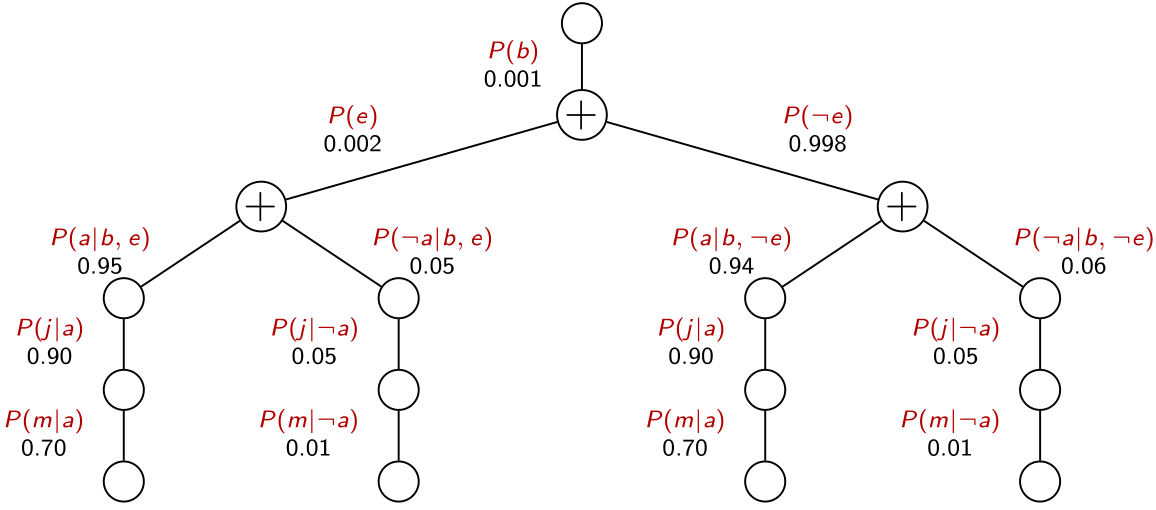
\includegraphics[width=0.75\textwidth]{img/img12.png}
\end{center} \vspace{3.5pt}
Despite these changes, the complexity of the expression is exponential, $O(2^n)$ - better than $O(n2^n)$, but still quite huge. The main reason complexity is still exponential
is attributable to the presence of repeated computation, or better, the products $P(j|a)P(m|a)$ and $P(j|\neg a)P(m|\neg a)$ are computed twice, once for each value of $e$.